\documentclass[border=8pt]{standalone}

\usepackage{tikz}
\usetikzlibrary{arrows.meta, positioning, calc, backgrounds}
\usepackage{xcolor}
\usepackage[T1]{fontenc}
\usepackage{helvet}
\renewcommand{\familydefault}{\sfdefault}

\definecolor{UniversityBlue}{HTML}{011451}

% Last node of the vertical chain. The sidebar fill, the "Analytic Sample"
% band midpoint and the footnote anchor all follow it, so re-enabling the
% mice / gFormulaMI boxes (E, F) for the paper is a one-line change here.
\newcommand{\lastnode}{D}   % <- set to F when E and F are uncommented

\tikzset{
  mainbox/.style={
    rectangle, draw=black, line width=0.5pt,
    minimum width=7.5cm, text width=7.1cm,
    align=center, font=\small, fill=white, inner sep=8pt
  },
  sidebox/.style={
    rectangle, draw=black, line width=0.5pt,
    minimum width=5.5cm, text width=5.1cm,
    align=center, font=\small, fill=white, inner sep=8pt
  },
  arrow/.style={
    -{Latex[length=6pt, width=5pt]},
    line width=0.8pt
  }
}

\begin{document}
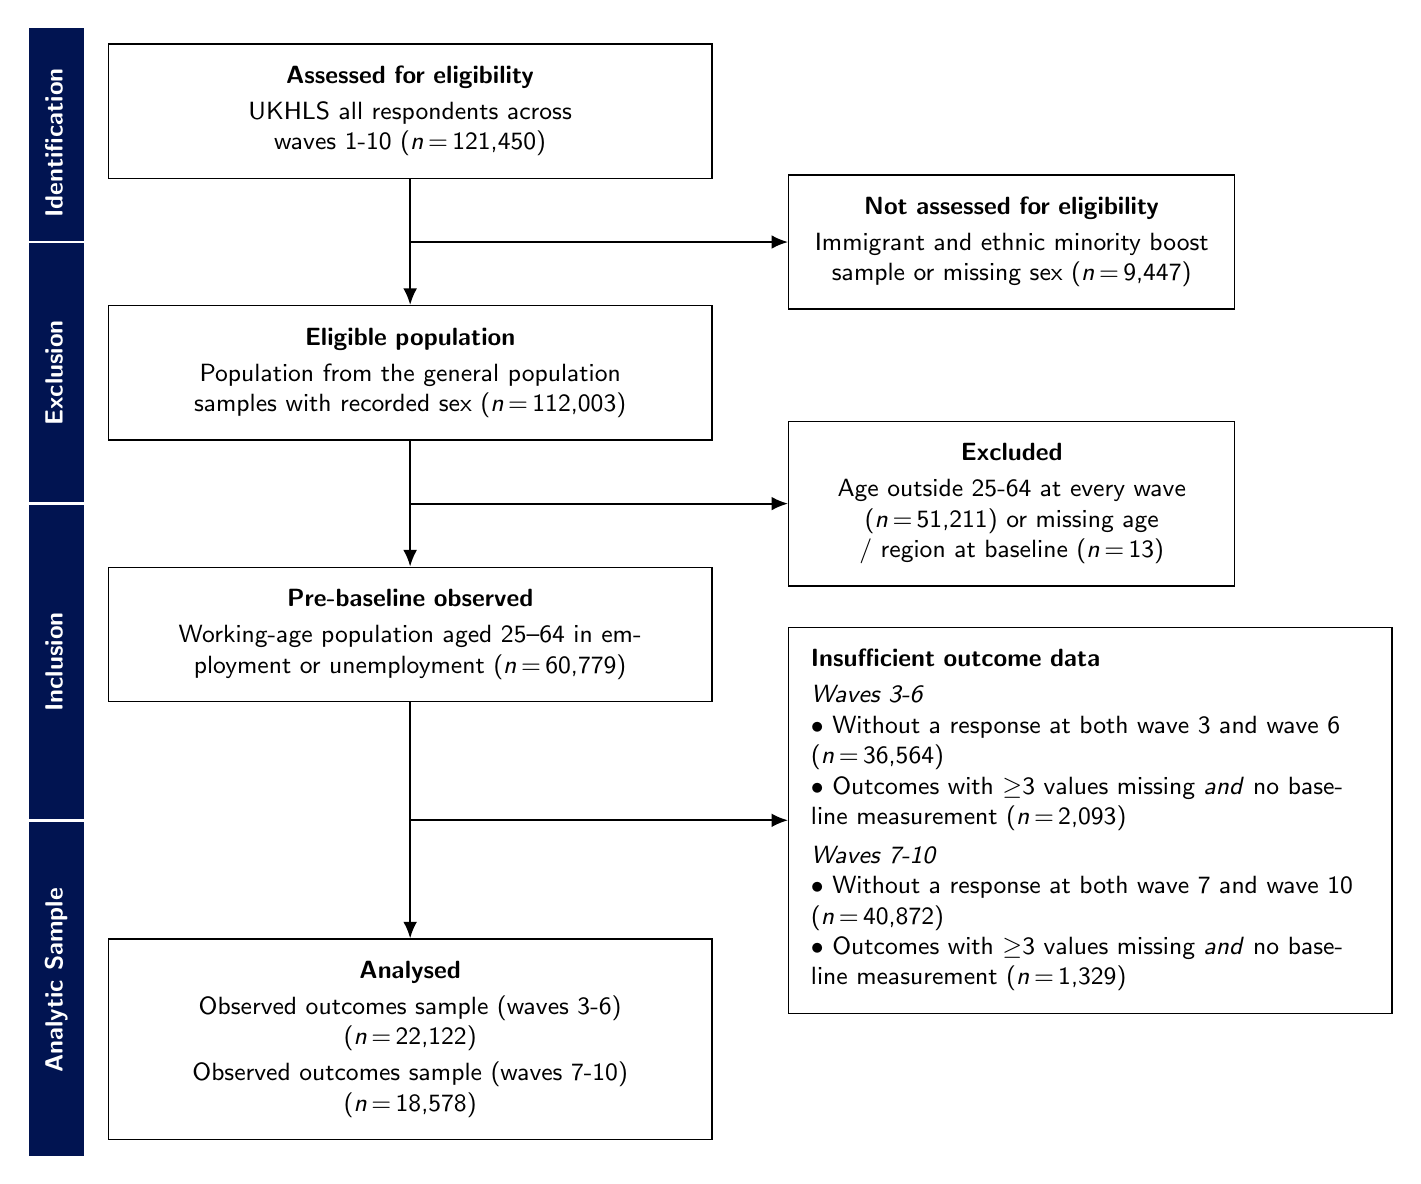
\begin{tikzpicture}

% ── Main flow boxes ───────────────────────────────────────────────────────────

\node[mainbox] (A) {%
  \textbf{Assessed for eligibility}\\[2pt]
  UKHLS all respondents across waves 1-10 (\emph{n}\,=\,121,450)
};

\node[mainbox, below=1.6cm of A] (B) {%
  \textbf{Eligible population}\\[2pt]
  Population from the general population samples with recorded sex (\emph{n}\,=\,112,003)
};

\node[mainbox, below=1.6cm of B] (C) {%
  \textbf{Pre-baseline observed}\\[2pt]
  Working-age population aged 25--64 in employment or unemployment (\emph{n}\,=\,60,779)
};

\node[mainbox, below=3.0cm of C] (D) {%
  \textbf{Analysed}\\[2pt]
  Observed outcomes sample (waves 3-6) \\
  (\emph{n}\,=\,22,122) \\[2pt]
  Observed outcomes sample (waves 7-10) \\
  (\emph{n}\,=\,18,578)
};

% \node[mainbox, below=1.6cm of D] (E) {%
%  \textbf{Multiple imputation of observed outcomes}\\[2pt]
%  Observed cases imputed to generate complete datasets (\emph{M}\,=\,75 imputations)
%};

%\node[mainbox, below=1.6cm of E] (F) {%
%  \textbf{Multiple imputation of potential outcomes}\\[2pt]
%  Imputed datasets introduced to generate potential outcomes datasets for g-formula estimation (\emph{M}\,=\,75 imputations)
%};

% ── Gap midpoints (on the vertical connecting arrows) ─────────────────────────

\coordinate (mAB) at ($(A.south)!0.5!(B.north)$);
\coordinate (mBC) at ($(B.south)!0.5!(C.north)$);
\coordinate (mCD) at ($(C.south)!0.5!(D.north)$);

% ── Exclusion boxes — anchored at gap midpoints for clean horizontal arrows ───

\node[sidebox, anchor=west] (excl1) at ($(mAB) + (4.8cm, 0)$) {%
  \textbf{Not assessed for eligibility}\\[2pt]
  Immigrant and ethnic minority boost sample or missing sex (\emph{n}\,=\,9,447)
};

\node[sidebox, anchor=west] (excl2) at ($(mBC) + (4.8cm, 0)$) {%
  \textbf{Excluded}\\[2pt]
  Age outside 25-64 at every wave (\emph{n}\,=\,51,211) or missing age / region at baseline (\emph{n}\,=\,13)
};

\node[sidebox, align=left, text width=7.1cm, minimum width=7.5cm, anchor=west] (excl3) at ($(mCD) + (4.8cm, 0)$) {%
  \textbf{Insufficient outcome data}\\[2pt]
  \emph{Waves 3-6}\\
  $\bullet$ Without a response at both wave~3 and wave~6 (\emph{n}\,=\,36,564)\\
  $\bullet$ Outcomes with ${\geq}$3 values missing \emph{and} no baseline measurement (\emph{n}\,=\,2,093)\\[3pt]
  \emph{Waves 7-10}\\
  $\bullet$ Without a response at both wave~7 and wave~10 (\emph{n}\,=\,40,872)\\
  $\bullet$ Outcomes with ${\geq}$3 values missing \emph{and} no baseline measurement (\emph{n}\,=\,1,329)
};

% ── Main vertical arrows ──────────────────────────────────────────────────────

\draw[arrow] (A.south) -- (B.north);
\draw[arrow] (B.south) -- (C.north);
\draw[arrow] (C.south) -- (D.north);
%\draw[arrow] (D.south) -- node[right, font=\small\itshape, xshift=3pt] {mice} (E.north);
%\draw[arrow] (E.south) -- node[right, font=\small\itshape, xshift=3pt] {gFormulaMI} (F.north);

% ── Exclusion arrows — purely horizontal from gap midpoints ──────────────────

\draw[arrow] (mAB) -- (excl1.west);
\draw[arrow] (mBC) -- (excl2.west);
\draw[arrow] (mCD) -- (excl3.west);

% ── Sidebar: single navy fill + white dividers (no separate label boxes) ──────

% Sidebar geometry: spans from 1.0cm left of A.west to 0.3cm left of A.west
\coordinate (sideL) at ($(A.west) + (-1.0cm, 0)$);
\coordinate (sideR) at ($(A.west) + (-0.3cm, 0)$);
\coordinate (sideC) at ($(A.west) + (-0.65cm, 0)$);

% Section vertical centres (for rotated text placement)
\coordinate (cID) at ($(A.north)!0.5!(mAB)$);
\coordinate (cEX) at ($(mAB)!0.5!(mBC)$);
\coordinate (cIN) at ($(mBC)!0.5!(mCD)$);
\coordinate (cAN) at ($(mCD)!0.5!(\lastnode.south)$);

\begin{scope}[on background layer]
  % Continuous navy rectangle spanning full height
  \fill[UniversityBlue]
    ($(A.north -| sideL) + (0, 0.2cm)$) rectangle
    ($(\lastnode.south -| sideR) + (0, -0.2cm)$);

  % White dividers between sections
  \draw[white, line width=1pt] (sideL |- mAB) -- (sideR |- mAB);
  \draw[white, line width=1pt] (sideL |- mBC) -- (sideR |- mBC);
  \draw[white, line width=1pt] (sideL |- mCD) -- (sideR |- mCD);
\end{scope}

% Section labels (rotated text, centred in each section)
\node[text=white, font=\small\bfseries, rotate=90] at (sideC |- cID) {\strut Identification};
\node[text=white, font=\small\bfseries, rotate=90] at (sideC |- cEX) {\strut Exclusion};
\node[text=white, font=\small\bfseries, rotate=90] at (sideC |- cIN) {\strut Inclusion};
\node[text=white, font=\small\bfseries, rotate=90] at (sideC |- cAN) {\strut Analytic Sample};

% ── Footnote ──────────────────────────────────────────────────────────────────

%\node[
%  below=0.5cm of \lastnode,
%  anchor=north,
%  text width=13cm,
%  align=justify,
%  font=\footnotesize
%] {%
%  \textsuperscript{a}\,Age was imputed by carrying forward the baseline (wave~1) age value and incrementing it by one year per subsequent wave.
%};

\end{tikzpicture}
\end{document}
